\subsection{Share of Detected Cases}
\label{subsec:data_share_known_cases}

\begin{figure}[ht]
  \centering
  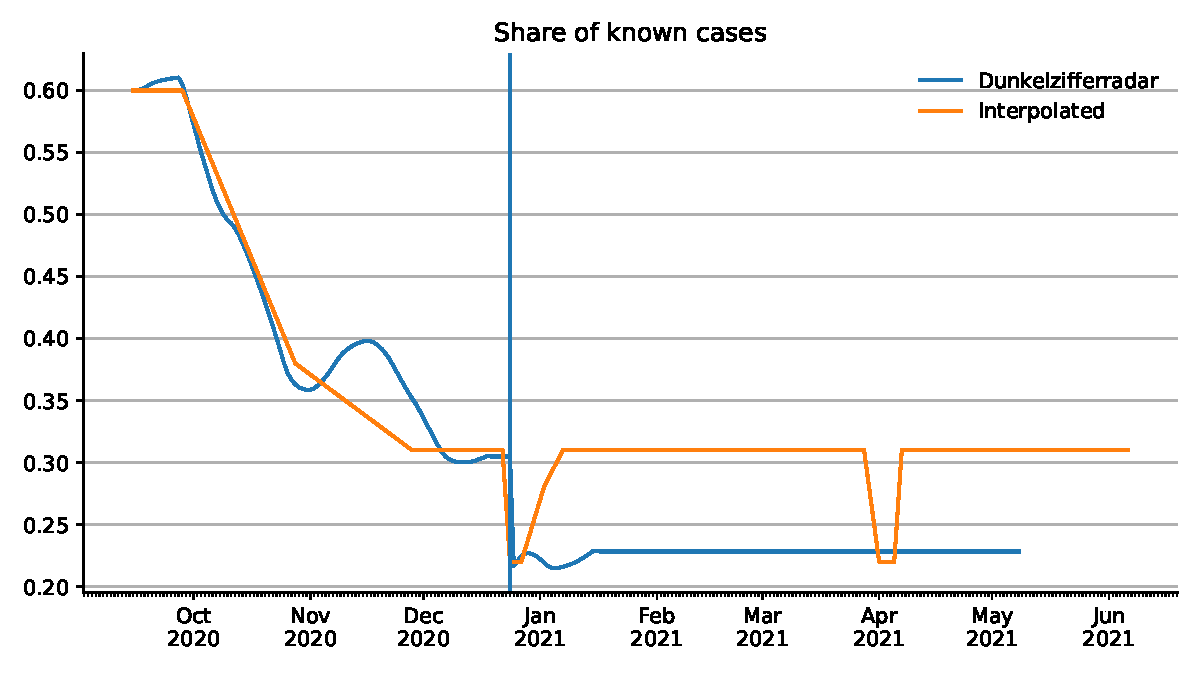
\includegraphics[width=\textwidth]{figures/results/figures/data/testing/assumed_overall_share_known_cases}
  \caption{Share of Detected Cases}
  \label{fig:share_known_cases_data}
  \floatfoot{\noindent \textit{Note:} The figure shows the share of cases that is
  reported as an official case via PCR confirmation. We use the overall share of known
  cases that was estimated through the case fatality ratio by the
  \href{https://covid19.dunkelzifferradar.de/}{Dunkelzifferradar} for all of 2020 and
  then assume it to be constant as vaccinations of the elderly strongly affect the case
  fatality rate which the project does not account for. Starting in 2021 in addition to
  the overall numbers of detected cases through symptoms and the share known cases, cases
  are also detected through confirmation of positive rapid tests which happens
  endogenously inside the model. For the public holidays of Christmas and Easter we lower
  the share of detected cases as fewer PCR tests are available during public holidays.}
\end{figure}

\FloatBarrier